% !TEX program = pdflatex
% AIAA Regional Student Conference Format
\documentclass[conf]{new-aiaa}

\let\Bbbk\relax
\usepackage{amsmath,amssymb,amsfonts}
\usepackage{algorithm}
\usepackage{algorithmic}
\usepackage{booktabs}
\usepackage{graphicx}
\usepackage{authblk}
\usepackage{hyperref}
\usepackage{tikz}
\usetikzlibrary{arrows.meta,positioning,shapes.geometric,fit,calc}
\usepackage{pgfplots}
\pgfplotsset{compat=1.18}
\hypersetup{colorlinks=true,linkcolor=blue,citecolor=blue,urlcolor=blue}

\title{Human-Supervised CFAR Autotuning for Maritime Sensing}

\author{Nathan Kirk\footnote{Undergraduate Student, Department of Mechanical Engineering, AIAA Student Member, Member ID: 1924156.}}
\author{J.C. Vaught\footnote{Graduate Student, Department of Mechanical Engineering, AIAA Student Member, Member ID: 1537189.}}
\author{Douglas Cahl\footnote{Professor, Department of Mechanical Engineering.}}
\author{Yi Wang\footnote{Professor, Department of Mechanical Engineering.}}
\affil{University of South Carolina, Columbia, SC, 29208}

\date{}

\begin{document}
\maketitle

\begin{abstract}
Radar-based target detection in cluttered environments requires robust detection under tight size, weight, power, and cost constraints. Tuning Constant False Alarm Rate (CFAR) detectors for heterogeneous scenes is difficult due to heavy-tailed clutter, terrain transitions, and multipath, yet remains essential for low-latency situational awareness. We present a human-supervised methodology and open-source browser-based tool, \emph{CFAR Studio}, for tuning CFAR parameters of commercial-off-the-shelf radars. The operator annotates stationary reference objects on one or more radar frames using an interactive blob-tracing tool. The system then performs an exhaustive grid search over three CFAR variants -- Cell-Averaging (CA), Greatest-Of (GO), and Smallest-Of (SO) -- evaluating each parameter configuration against the annotated ground truth via an area-weighted coverage score. Multi-frame temporal stability is assessed by tracking detection consistency across sequential radar sweeps. An integral-image optimization enables the evaluation of hundreds of configurations in seconds entirely within the browser. The system is demonstrated on real X-band radar data collected with a Furuno NXT DRS4D radar and Raspberry Pi~5 at Lake Murray, South Carolina.
\end{abstract}

\section{Introduction}
Constant False Alarm Rate (CFAR) detectors are the dominant target-detection paradigm in radar systems, valued for their controllable false-alarm probability, local-statistics design, and suitability for embedded implementations \cite{farina2005review, gandhi1988}. Under homogeneous, Gaussian clutter the threshold multiplier admits a closed-form solution and detection performance is well characterized \cite{finn1968, richards2022}. Yet real-world environments violate every assumption this theory depends on -- clutter is heavy-tailed and spatially nonhomogeneous, well modeled by K-distribution and Pareto families rather than Rayleigh statistics \cite{ward2006, rosenberg2013}; terrain transition edges introduce abrupt power discontinuities; and multipath, mixed cooperative/non-cooperative traffic, and environmental returns further corrupt the reference window. As a result, selecting appropriate CFAR parameters is notoriously scene- and sensor-dependent -- a configuration that works in one region may generate excessive false alarms in another, while aggressive clutter rejection near terrain boundaries may mask small targets of interest \cite{dhs2009}. Currently, operators tune guard cells, reference windows, and false-alarm rates by manual trial-and-error, adjusting settings until the display ``looks right.'' This process is slow, subjective, and not reproducible.

Researchers have sought to address these limitations through adaptive and knowledge-based CFAR schemes. Variability-Index CFAR dynamically switches between CA, GO, and SO variants via hypothesis tests on the reference window \cite{smith2000}; knowledge-based detectors exploit GIS databases to select training samples appropriate to the local terrain \cite{farina2008kb}; and cognitive CFAR approaches compare local clutter statistics against prior performance models to adjust window length \cite{humphreys2022}. More recently, deep-learning detectors have demonstrated strong accuracy on radar data \cite{salalstm2023}. However, each approach carries practical constraints that limit operational adoption. Adaptive switching heuristics degrade when interfering targets span both halves of the reference window \cite{smith2000}. Knowledge-based methods require pre-built environmental databases that do not exist for ad-hoc deployments in unfamiliar environments \cite{farina2008kb}. Cognitive CFAR optimizes window length alone, leaving the choice of variant, guard-cell size, and $P_{\mathrm{FA}}$ to the operator \cite{humphreys2022}. Deep-learning detectors abandon the CFAR property entirely, cannot guarantee false-alarm control, and require large labeled datasets that are unavailable in most operational settings \cite{cfarnet2024}. Despite decades of effort, no method systematically searches across multiple CFAR variants and the full parameter space to find the best configuration for a given scene.

The tooling landscape compounds the problem. Commercial radar processors from major vendors embed proprietary CFAR logic with limited or no parameter exposure, while third-party research tools that do expose the full parameter set -- most notably MATLAB's Radar Toolbox \cite{mathworksCFAR} -- require expensive licenses, desktop installations, and cannot be deployed on edge hardware or shared without infrastructure. Yet field operators, small teams, and academic researchers -- the users who most need tunable detection for challenging scenes -- are precisely those without access to these toolchains. No open, installation-free tool exists that allows an operator to experiment with CFAR configurations in situ.

A further gap lies in how CFAR configurations are evaluated. Standard assessment relies on probability-of-detection and probability-of-false-alarm curves computed against synthetic injected targets or single-frame detection counts \cite{richards2022, skolnik2008}. However, this ignores two operational realities. First, radar operators already possess direct situational awareness of which stationary objects -- towers, pylons, buildings, infrastructure -- should appear on the display. This knowledge constitutes a free, high-quality source of ground truth, yet no prior work formalizes operator annotation as a quantitative objective function for CFAR optimization. Second, a configuration that detects a target on one sweep but loses it on the next is operationally useless for tracking and situational awareness; nevertheless, temporal consistency across sequential radar sweeps is absent from standard CFAR evaluation metrics.

This paper presents a human-supervised CFAR autotuning framework that addresses these gaps. The contributions are: (i)~a formal scoring function anchored to human-annotated ground-truth blobs, using area-weighted coverage ratios rather than binary detection indicators; (ii)~an exhaustive grid search over three CFAR variants (CA, GO, SO) with integral-image loop hoisting that enables evaluation of hundreds of configurations in seconds; (iii)~a multi-frame temporal stability metric that quantifies detection consistency across sequential radar sweeps; and (iv)~an open-source, fully client-side browser-based tool, \emph{CFAR Studio}, that requires no installation, server infrastructure, or specialized hardware beyond a modern web browser. The system is demonstrated on real X-band radar data collected with a Furuno DRS4D-NXT radar and Raspberry Pi~5 at Lake Murray, South Carolina.

\begin{figure*}[t]
    \centering
    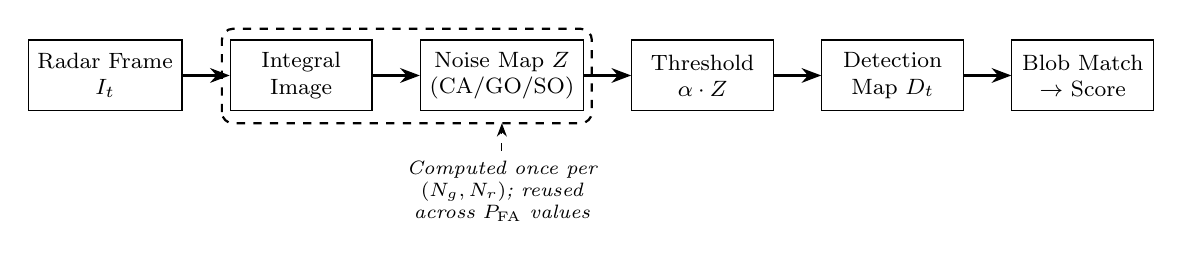
\begin{tikzpicture}[
        block/.style={rectangle, draw, minimum height=0.9cm, minimum width=1.8cm, align=center, font=\footnotesize},
        arrow/.style={-{Stealth[length=2.5mm]}, thick},
        note/.style={font=\scriptsize\itshape, text width=2.8cm, align=center}
    ]
        % Blocks
        \node[block] (frame) {Radar Frame\\$I_t$};
        \node[block, right=0.6cm of frame] (integral) {Integral\\Image};
        \node[block, right=0.6cm of integral] (noise) {Noise Map $Z$\\(CA/GO/SO)};
        \node[block, right=0.6cm of noise] (thresh) {Threshold\\$\alpha \cdot Z$};
        \node[block, right=0.6cm of thresh] (detect) {Detection\\Map $D_t$};
        \node[block, right=0.6cm of detect] (score) {Blob Match\\$\rightarrow$ Score};

        % Arrows
        \draw[arrow] (frame) -- (integral);
        \draw[arrow] (integral) -- (noise);
        \draw[arrow] (noise) -- (thresh);
        \draw[arrow] (thresh) -- (detect);
        \draw[arrow] (detect) -- (score);

        % Loop hoisting annotation
        \node[note, below=0.5cm of noise] (loopnote) {Computed once per $(N_g, N_r)$; reused across $P_{\mathrm{FA}}$ values};
        \draw[dashed, thick, rounded corners] ($(integral.south west)+(-0.1,-0.15)$) rectangle ($(noise.south east)+(0.1,1.05)$);
        \draw[-{Stealth}, dashed] (loopnote.north) -- ($(noise.south)+(0,-0.15)$);
    \end{tikzpicture}
    \caption{CFAR detection pipeline for a single parameter configuration. The noise map depends only on guard and reference cell counts, enabling \emph{loop hoisting}: for each $(N_g, N_r)$ pair, the noise map is computed once and reused across all $P_{\mathrm{FA}}$ values, reducing redundant computation.}
    \label{fig:cfar_pipeline}
\end{figure*}

\section{Background and Related Work}
The CA-CFAR family estimates background power via local training windows and compares the cell-under-test to a scaled noise estimate to maintain a desired $P_{\mathrm{FA}}$ \cite{finn1968, gandhi1988}. For $N$ independent, identically distributed reference cells drawn from an exponential background, the threshold multiplier admits the closed-form expression \cite{richards2022, finn1968}:
\begin{equation}
    \alpha = N\!\left(P_{\mathrm{FA}}^{-1/N} - 1\right). \label{eq:alpha}
\end{equation}
GO- and SO-CFAR improve robustness near clutter edges and in multi-target scenes by partitioning leading and trailing reference windows and selecting the greatest-of or smallest-of their respective noise estimates \cite{hansen1972, trunk1978}. Other variants -- including Order-Statistic (OS-CFAR), Variability-Index, and censored/trimmed-mean CFAR -- address additional heterogeneous-background scenarios \cite{farina2005review} but are beyond the scope of the current implementation.

High-resolution radar clutter is heavy-tailed and spatially nonhomogeneous. The K-distribution, a compound Gaussian model with gamma-distributed texture, has been widely adopted since Ward et al.\ \cite{ward2006}; however, Fioranelli et al.\ \cite{rosenberg2013} showed that Pareto-plus-noise models better capture the spiky returns observed at high grazing angles in X-band data. Comparative studies across 1--10\,GHz confirm that no single distribution fits all polarizations, resolutions, and sea states \cite{angelliaume2019}. These non-Gaussian, site-specific statistics are particularly problematic for CFAR detectors. Training windows that span terrain transitions or nearby infrastructure can severely bias noise estimates, inflating or suppressing the detection threshold in ways that the closed-form $\alpha$ cannot anticipate.

Several lines of work have sought to automate CFAR parameter selection. Humphreys et al.\ \cite{humphreys2022} proposed a cognitive CFAR that adapts window length by comparing local statistics against prior performance models, but the approach does not address variant selection, guard-cell sizing, or $P_{\mathrm{FA}}$. Variability-Index CFAR \cite{smith2000} switches dynamically among CA, GO, and SO modes via hypothesis tests on the reference window; yet detection probability degrades when interfering targets are not confined to a single half-window. Neural-network-based variant selectors \cite{nncfar2019} and CFAR-constrained deep-learning detectors \cite{cfarnet2024} have shown accuracy improvements in simulation, but require offline training data, GPU infrastructure, and retraining when the sensor or scene changes. Cross-sensor supervision using lidar has been explored for automotive radar \cite{seefurther2024}; however, synchronized lidar is unavailable on most platforms and the resulting detector abandons the CFAR property entirely.

Despite these advances, we are not aware of prior work that jointly searches over CFAR variant, guard cells, reference cells, and $P_{\mathrm{FA}}$ using human-annotated ground truth as the objective function. Knowledge-based CFAR schemes \cite{farina2008kb} leverage GIS databases but require pre-built environmental maps unavailable for ad-hoc deployments. Expert-system approaches \cite{wicks1996} automate the operator out of the loop rather than harnessing operator situational awareness. Our approach treats the operator's annotation of stationary reference objects as quantitative ground truth, defining a formal objective function that the system optimizes via exhaustive search -- combining human judgment with computational efficiency in a browser-deployable tool.

\begin{figure}[t]
    \centering
    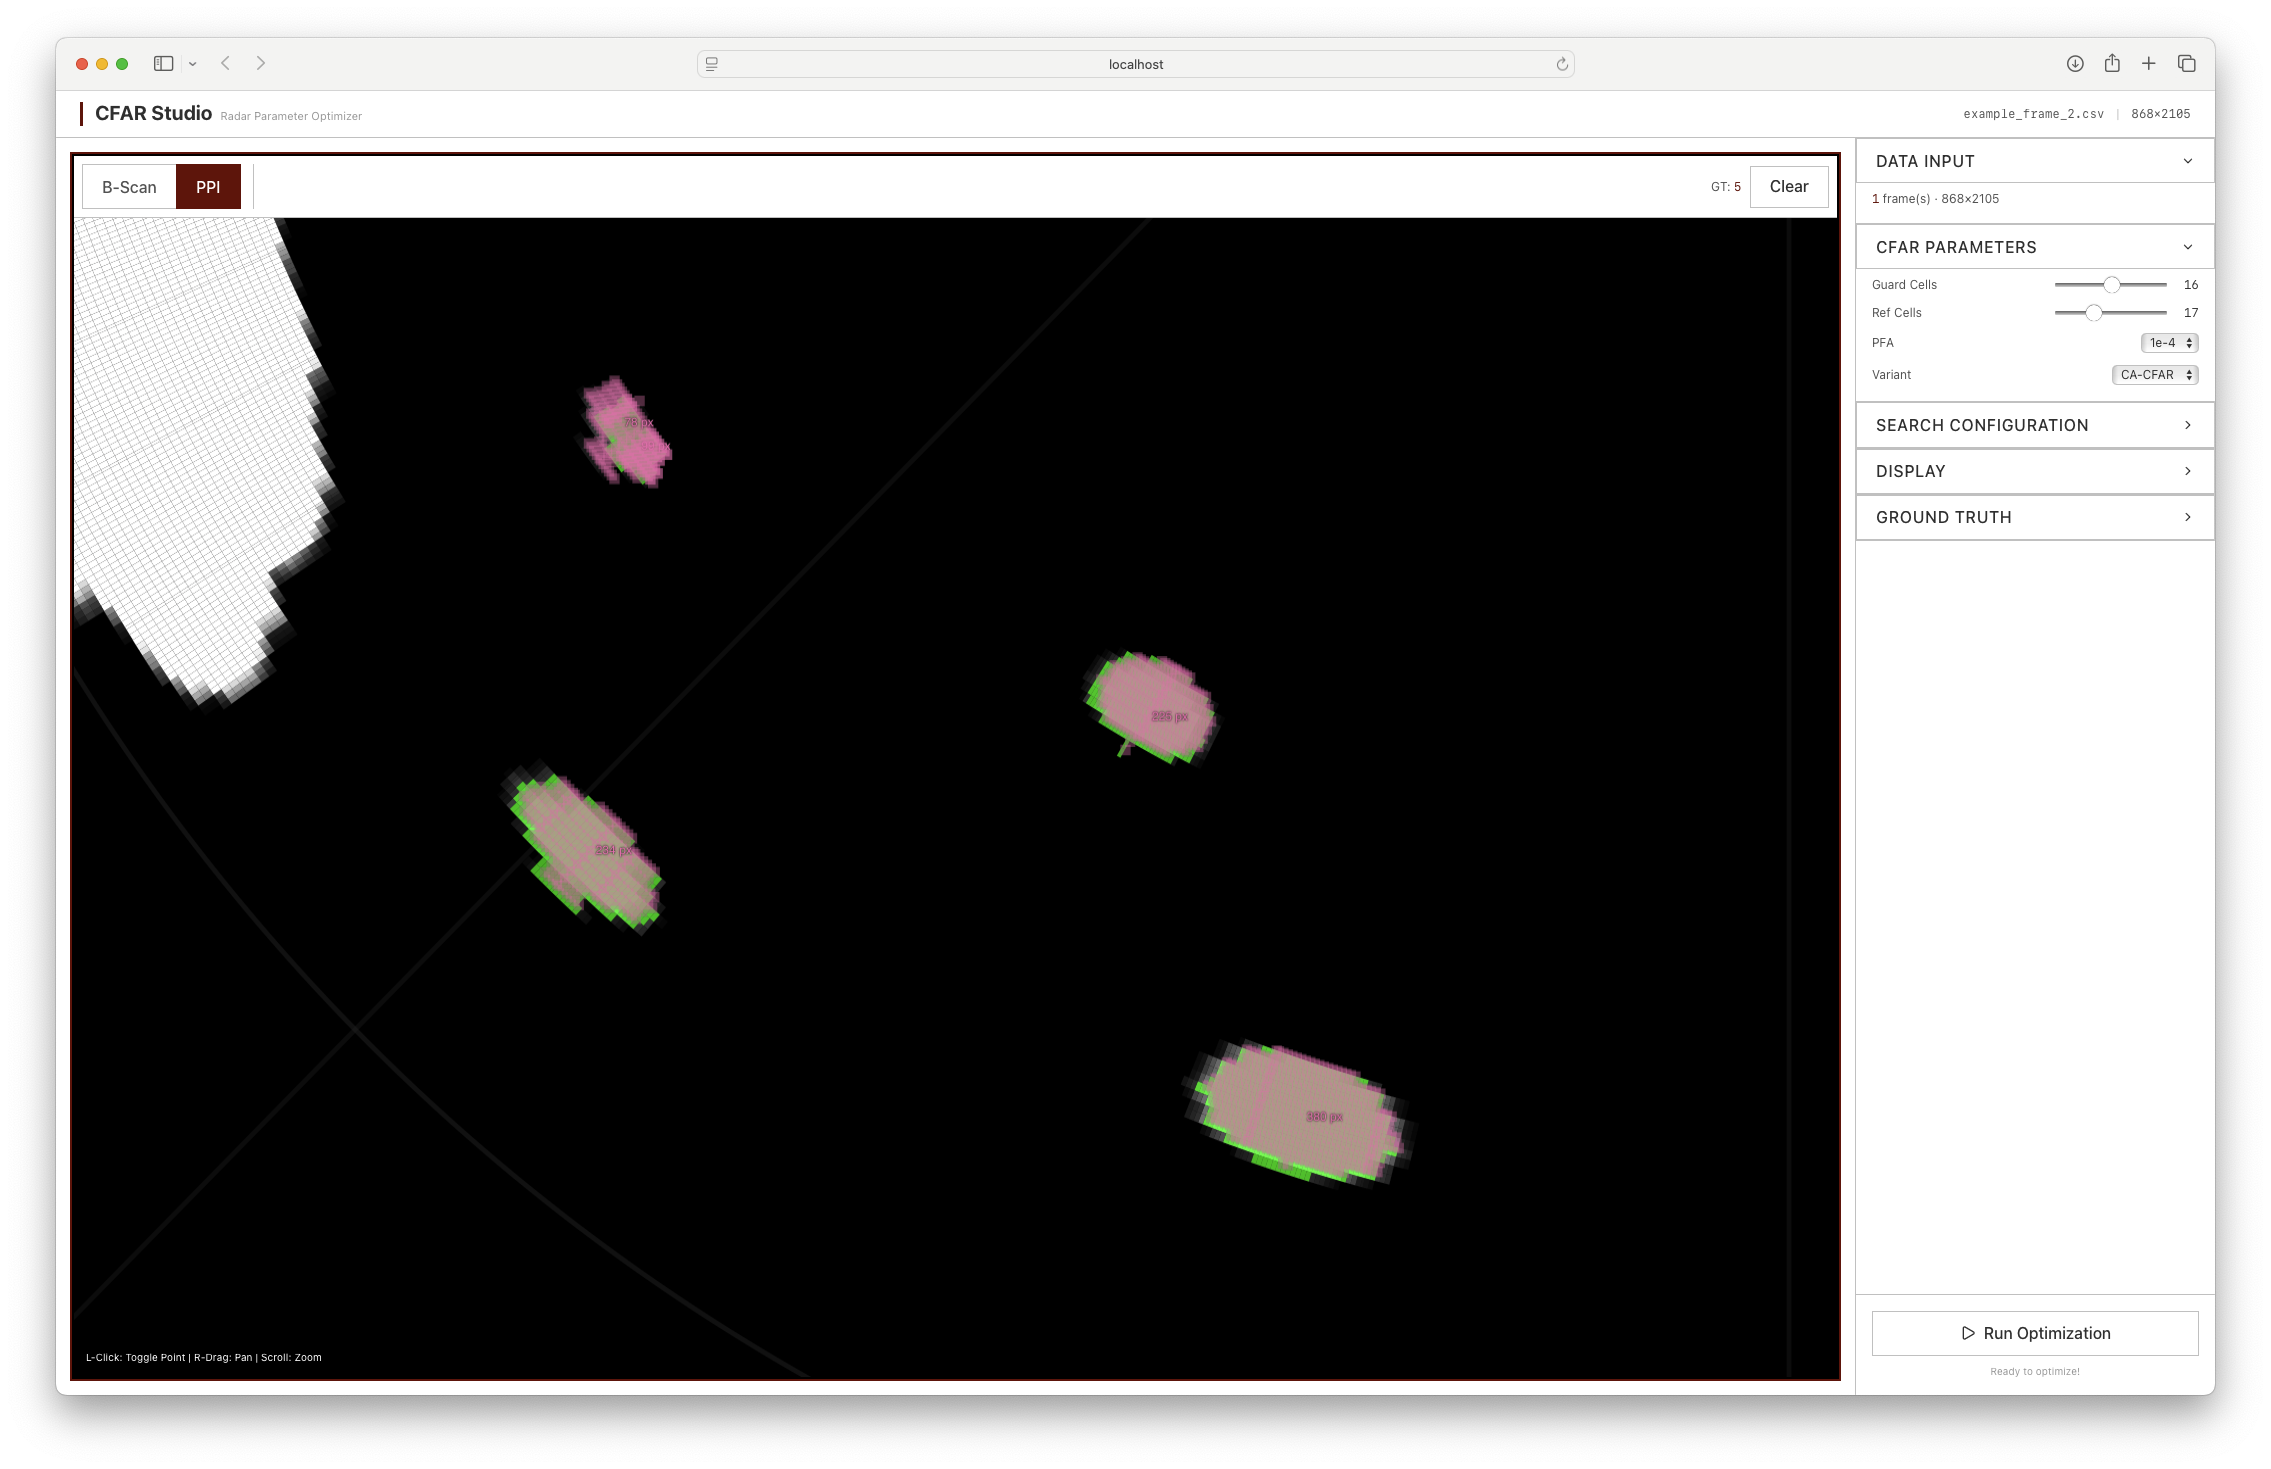
\includegraphics[width=\columnwidth]{figures/ppi_zoomed_ground_truth_annotations.png}
    \caption{Close-up of ground truth annotations on the PPI display. The operator clicks on a detected target; an 8-connected flood fill traces the contiguous detection blob, capturing its exact pixel footprint as the reference shape for scoring.}
    \label{fig:ground_truth}
\end{figure}

\section{Problem Formulation}

Let $I_t \in \mathbb{R}^{M\times N}$ denote radar intensity frames in range--azimuth coordinates, $t = 1,\dots,T$. A CFAR variant $v \in \{$CA, GO, SO$\}$ with parameter vector $\boldsymbol{\theta} = (N_g, N_r, P_{\mathrm{FA}})$ -- guard cells, reference cells, and probability of false alarm -- is applied to each frame to produce a binary detection map $D_t(v, \boldsymbol{\theta}) \in \{0,1\}^{M\times N}$.

\label{sec:cfar_detection}

\subsection{CFAR Detection Variants}

All three variants considered in this work -- CA, GO, and SO -- share a common two-dimensional sliding-window architecture applied independently to each pixel of the radar frame. For a given cell-under-test at pixel $(i,j)$ in frame $I_t$, the detector defines two concentric rectangular regions: a \emph{guard region} of half-width $N_g$ that excludes the cell-under-test and its immediate neighbors from the noise estimate, and a \emph{reference annulus} of width $N_r$ that surrounds the guard region and provides the training samples from which the local noise level is estimated. The guard region prevents the target's own energy from inflating the noise estimate, while the reference annulus should be large enough to yield a statistically reliable background estimate yet small enough to remain within a locally homogeneous clutter region. To avoid the computational cost of summing over the reference annulus at every pixel, the implementation pre-computes an integral image (summed area table) \cite{crow1984} for each frame, enabling $O(1)$ evaluation of the sum over any axis-aligned rectangular region. With the integral image in place, the three variants differ only in how they aggregate the reference cells into a single noise estimate $Z_{i,j}$.

\begin{figure}[t]
    \centering
    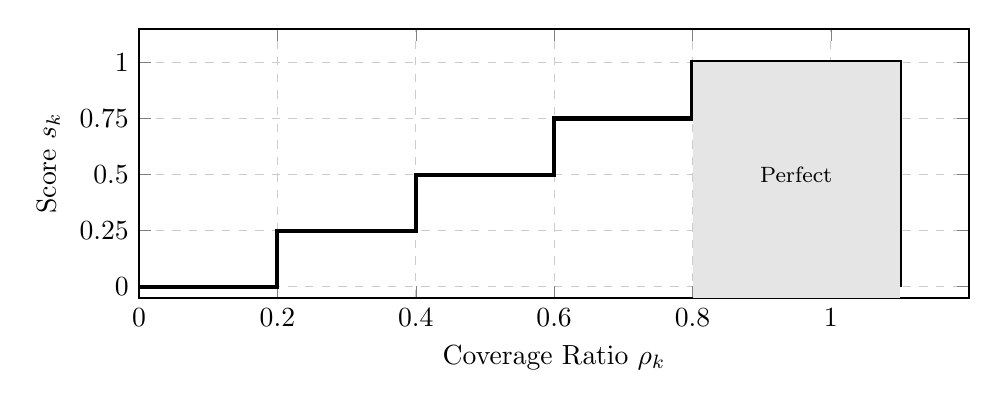
\begin{tikzpicture}
        \begin{axis}[
            width=\columnwidth,
            height=5cm,
            xlabel={Coverage Ratio $\rho_k$},
            ylabel={Score $s_k$},
            xmin=0, xmax=1.2,
            ymin=-0.05, ymax=1.15,
            xtick={0, 0.2, 0.4, 0.6, 0.8, 1.0},
            ytick={0, 0.25, 0.5, 0.75, 1.0},
            grid=major,
            grid style={dashed, gray!40},
            thick,
            every axis plot/.append style={line width=1.5pt},
        ]
            % Step function
            \addplot[const plot, color=black, line width=1.5pt] coordinates {
                (0, 0) (0.2, 0.25) (0.4, 0.5) (0.6, 0.75) (0.8, 1.0) (1.1, 0)
            };
            % Shade the perfect zone
            \fill[black!10] (axis cs:0.8,-0.05) rectangle (axis cs:1.1,1.0);
            \node[font=\footnotesize] at (axis cs:0.95,0.5) {Perfect};
        \end{axis}
    \end{tikzpicture}
    \caption{Scoring function mapping area coverage ratio $\rho_k$ to discrete score $s_k$. Configurations that capture 80--110\% of the ground truth blob area receive a perfect score; partial detections are penalized proportionally.}
    \label{fig:scoring_function}
\end{figure}

\subsubsection{CA-CFAR}
Cell-Averaging CFAR computes the arithmetic mean of all $N = (2R_o+1)^2 - (2R_i+1)^2$ reference cells, where $R_o = N_g + N_r$ is the outer half-width and $R_i = N_g$ is the inner half-width:
\begin{equation}
    Z_{i,j}^{\mathrm{CA}} = \frac{1}{N}\left(S_{\mathrm{outer}} - S_{\mathrm{inner}}\right), \label{eq:ca}
\end{equation}
where $S_{\mathrm{outer}}$ and $S_{\mathrm{inner}}$ are the summed-area-table queries over the outer and inner rectangles, respectively. CA-CFAR is optimal under homogeneous, exponentially distributed clutter but can suffer threshold elevation when strong interferers or clutter edges fall within the reference annulus.

\subsubsection{GO-CFAR}
Greatest-Of CFAR mitigates the clutter-edge problem by splitting the reference annulus into two half-windows -- one leading (above) and one trailing (below) the cell-under-test -- and selecting the larger of the two noise estimates. Let $\bar{Z}_1$ and $\bar{Z}_2$ denote the mean power of each half-window, each containing $N_{\mathrm{half}}$ cells:
\begin{equation}
    Z_{i,j}^{\mathrm{GO}} = \max(\bar{Z}_1, \bar{Z}_2). \label{eq:go}
\end{equation}
By adopting the higher noise estimate, GO-CFAR raises the threshold near clutter transitions, suppressing false alarms at the cost of reduced detection sensitivity for weak targets.

\subsubsection{SO-CFAR}
Smallest-Of CFAR takes the opposite approach, selecting the lower of the two half-window estimates:
\begin{equation}
    Z_{i,j}^{\mathrm{SO}} = \min(\bar{Z}_1, \bar{Z}_2). \label{eq:so}
\end{equation}
This preserves sensitivity near clutter edges -- useful for detecting targets that lie adjacent to terrain or structures -- but at the expense of an elevated false-alarm rate in heterogeneous regions where the quieter half-window underestimates the true background.

For both GO- and SO-CFAR, the effective reference cell count used for the threshold multiplier $\alpha$ (Eq.~\ref{eq:alpha}) is $N_{\mathrm{half}}$ rather than the full annulus count $N$, reflecting the reduced number of independent training samples.



\begin{algorithm}[t]
\caption{Grid Search with Loop Hoisting}
\label{alg:grid_search}
\begin{algorithmic}[1]
\STATE \textbf{Input:} frames $\{I_t\}_{t=1}^T$, ground truth blobs $\{\mathcal{B}_k\}$, variant $v$, parameter ranges
\STATE Pre-compute integral images for all frames
\FOR{each $(N_g, N_r)$ in parameter grid}
    \STATE Compute noise map $Z$ for all frames \hfill $\triangleright$ \emph{Expensive step}
    \FOR{each $P_{\mathrm{FA}}$ value}
        \STATE $\alpha \leftarrow N_{\mathrm{eff}}(P_{\mathrm{FA}}^{-1/N_{\mathrm{eff}}} - 1)$
        \STATE Apply threshold: $D_t(i,j) \leftarrow \mathbb{1}[I_t(i,j) > \alpha \cdot Z_{i,j}]$
        \STATE Compute coverage scores $\{s_k\}$, frame score, false alarms, stability
    \ENDFOR
\ENDFOR
\STATE \textbf{Return} all results sorted by score
\end{algorithmic}
\end{algorithm}


\subsection{Detection Rule}

Given the noise estimate from any of the three variants, a detection is declared when the cell-under-test exceeds the scaled noise floor:
\begin{equation}
    D_t(i,j) = \mathbb{1}\!\left[I_t(i,j) > \alpha \cdot Z_{i,j}\right], \label{eq:detection}
\end{equation}
where the threshold multiplier $\alpha$ is given by Eq.~\eqref{eq:alpha} using the appropriate effective cell count. The resulting binary detection map $D_t$ is then evaluated against the operator's ground truth annotations as described in the following subsections.

\label{sec:ground_truth}

The operator annotates stationary reference objects (e.g., towers, buildings, infrastructure) on the radar PPI display. When the operator clicks on a detected pixel, an 8-connected flood-fill algorithm traces the contiguous detection blob $\mathcal{B}_k$, collecting all connected pixels into a set of indices. This ``magic wand'' approach captures the exact shape and area of each reference object as it appears in the current CFAR detection, rather than requiring the operator to draw bounding boxes or estimate target extent. The resulting blob pixel set $\mathcal{B}_k = \{p_1, p_2, \dots, p_{|\mathcal{B}_k|}\}$ serves as the ground truth reference for scoring.

\label{sec:scoring}

For each ground truth blob $\mathcal{B}_k$ and a candidate detection map $D_t$, we compute the \emph{area coverage ratio}:
\begin{equation}
    \rho_k = \frac{\sum_{p \in \mathcal{B}_k} D_t(p)}{|\mathcal{B}_k|}. \label{eq:coverage}
\end{equation}

This ratio measures what fraction of the ground truth blob's pixels are detected by the candidate configuration. The coverage ratio is mapped to a discrete score via a piecewise function that rewards configurations capturing the full target shape:

\begin{equation}
    s_k = \begin{cases}
        1.00 & \text{if } 0.8 \le \rho_k \le 1.1, \\
        0.75 & \text{if } 0.6 \le \rho_k < 0.8, \\
        0.50 & \text{if } 0.4 \le \rho_k < 0.6, \\
        0.25 & \text{if } 0.2 \le \rho_k < 0.4, \\
        0.00 & \text{if } \rho_k < 0.2.
    \end{cases} \label{eq:score_zones}
\end{equation}


The upper bound of 1.1 accommodates slight detection expansion beyond the annotated blob boundary, which is common when a slightly more sensitive configuration captures peripheral pixels. This area-based approach provides substantially more nuance than a binary ``detected/not-detected'' metric; a configuration that detects only a small fragment of a large target is appropriately penalized, while one that captures the full target shape is rewarded.

The per-frame score across all $K$ ground truth targets combines the worst-case and average target scores:
\begin{equation}
    S_{\mathrm{frame}} = 0.7 \cdot \min_{k \in [K]} s_k + 0.3 \cdot \frac{1}{K}\sum_{k=1}^{K} s_k. \label{eq:frame_score}
\end{equation}
The heavy weighting on the minimum score (0.7) enforces a critical constraint -- a configuration that completely misses even one annotated target is severely penalized regardless of how well it detects the others. This prevents the optimizer from recommending configurations that sacrifice coverage of difficult targets in favor of easy ones. In addition to target coverage, the false alarm count is computed as the number of detected pixels that fall outside all ground truth blobs:
\begin{equation}
    \mathrm{FP} = \sum_{t=1}^{T}\left(\sum_{(i,j)} D_t(i,j) - \sum_{k=1}^{K}\sum_{p \in \mathcal{B}_k} D_t(p)\right). \label{eq:fp}
\end{equation}
This metric allows the operator to compare configurations that achieve similar coverage scores but differ in the number of spurious detections they produce.

\label{sec:stability}

When multiple sequential frames are available, temporal stability quantifies how consistently each target is detected across the frame sequence. For each ground truth target $k$, let $c_k$ be the number of frames in which it is detected (score $> 0$). The stability metric is
\begin{equation}
    \mathrm{Stability} = \frac{1}{K}\sum_{k=1}^{K} \frac{c_k}{T}. \label{eq:stability}
\end{equation}
A stability of 1.0 indicates that all targets are detected in every frame, while low stability reveals configurations that are marginally sensitive and produce intermittent detections -- a failure mode that is operationally unacceptable for tracking and situational awareness even if the single-frame score is high.

\label{sec:grid_search}

The parameter space is defined by discrete ranges for guard cells $N_g$, reference cells $N_r$, and a set of $P_{\mathrm{FA}}$ values, with all combinations evaluated exhaustively. The key computational optimization exploits the fact that the noise map $Z$ depends only on $(N_g, N_r, v)$ and not on $P_{\mathrm{FA}}$. By restructuring the search loop to iterate over $(N_g, N_r)$ in the outer loop and $P_{\mathrm{FA}}$ in the inner loop, the expensive noise map computation is performed once per $(N_g, N_r)$ pair and reused across all $P_{\mathrm{FA}}$ values (Fig.~\ref{fig:cfar_pipeline}). Within the inner loop, only the scalar multiplication $\alpha \cdot Z_{i,j}$ and comparison in Eq.~\eqref{eq:detection} are needed. This \emph{loop hoisting} reduces the total number of integral-image queries by a factor equal to the number of $P_{\mathrm{FA}}$ values tested.


%% ============================================================
%% SECTION 4: SYSTEM ARCHITECTURE
%% ============================================================
\section{System Architecture}

\begin{figure*}[t]
    \centering
    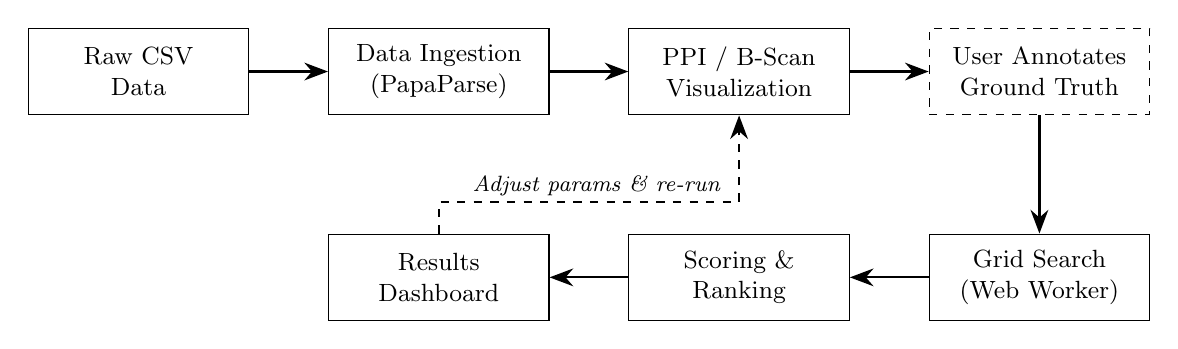
\begin{tikzpicture}[
        block/.style={rectangle, draw, minimum height=1.1cm, minimum width=2.8cm, align=center, font=\small},
        arrow/.style={-{Stealth[length=3mm]}, thick},
        userblock/.style={rectangle, draw, dashed, minimum height=1.1cm, minimum width=2.8cm, align=center, font=\small},
    ]
        % Row 1: Data ingestion and display
        \node[block] (csv) {Raw CSV\\Data};
        \node[block, right=1cm of csv] (parse) {Data Ingestion\\(PapaParse)};
        \node[block, right=1cm of parse] (viz) {PPI / B-Scan\\Visualization};
        \node[userblock, right=1cm of viz] (annotate) {User Annotates\\Ground Truth};

        % Row 2: Optimization (right to left, Grid Search under Annotate)
        \node[block, below=1.5cm of annotate] (worker) {Grid Search\\(Web Worker)};
        \node[block, left=1cm of worker] (scoring) {Scoring \&\\Ranking};
        \node[block, left=1cm of scoring] (results) {Results\\Dashboard};

        % Row 1 arrows
        \draw[arrow] (csv) -- (parse);
        \draw[arrow] (parse) -- (viz);
        \draw[arrow] (viz) -- (annotate);

        % Annotate straight down to Grid Search
        \draw[arrow] (annotate) -- (worker);

        % Row 2 arrows (right to left)
        \draw[arrow] (worker) -- (scoring);
        \draw[arrow] (scoring) -- (results);

        % Feedback loop: top of Results, right to under Viz, up into Viz bottom
        \draw[arrow, dashed] (results.north) -- ++(0,0.4) -| (viz.south);
        \node[font=\footnotesize\itshape] at ($(results.north)+(2.0,0.6)$) {Adjust params \& re-run};

    \end{tikzpicture}
    \caption{CFAR Studio system pipeline. Dashed box indicates user interaction; dashed arrow shows the iterative feedback loop where the operator can adjust parameters and re-run optimization after reviewing results.}
    \label{fig:pipeline}
\end{figure*}

CFAR Studio is implemented as a fully client-side web application using React~19 with TypeScript, built with Vite. All computation occurs in the user's browser with no server-side processing, no data upload, and no installation required. Plotly.js provides interactive PPI (Plan Position Indicator) and B-scan displays with multiple colormaps and zoom/pan controls. Radar CSV files are parsed via PapaParse, and a dedicated Web Worker thread performs the grid search without blocking the user interface.

Radar data is ingested from CSV files containing range--azimuth intensity matrices. Each CSV row corresponds to one azimuth spoke, with columns representing range bins. A companion azimuth array specifies the angular position of each spoke. The system supports multi-frame loading, enabling temporal analysis across sequential radar sweeps.

\begin{figure}[t]
    \centering
    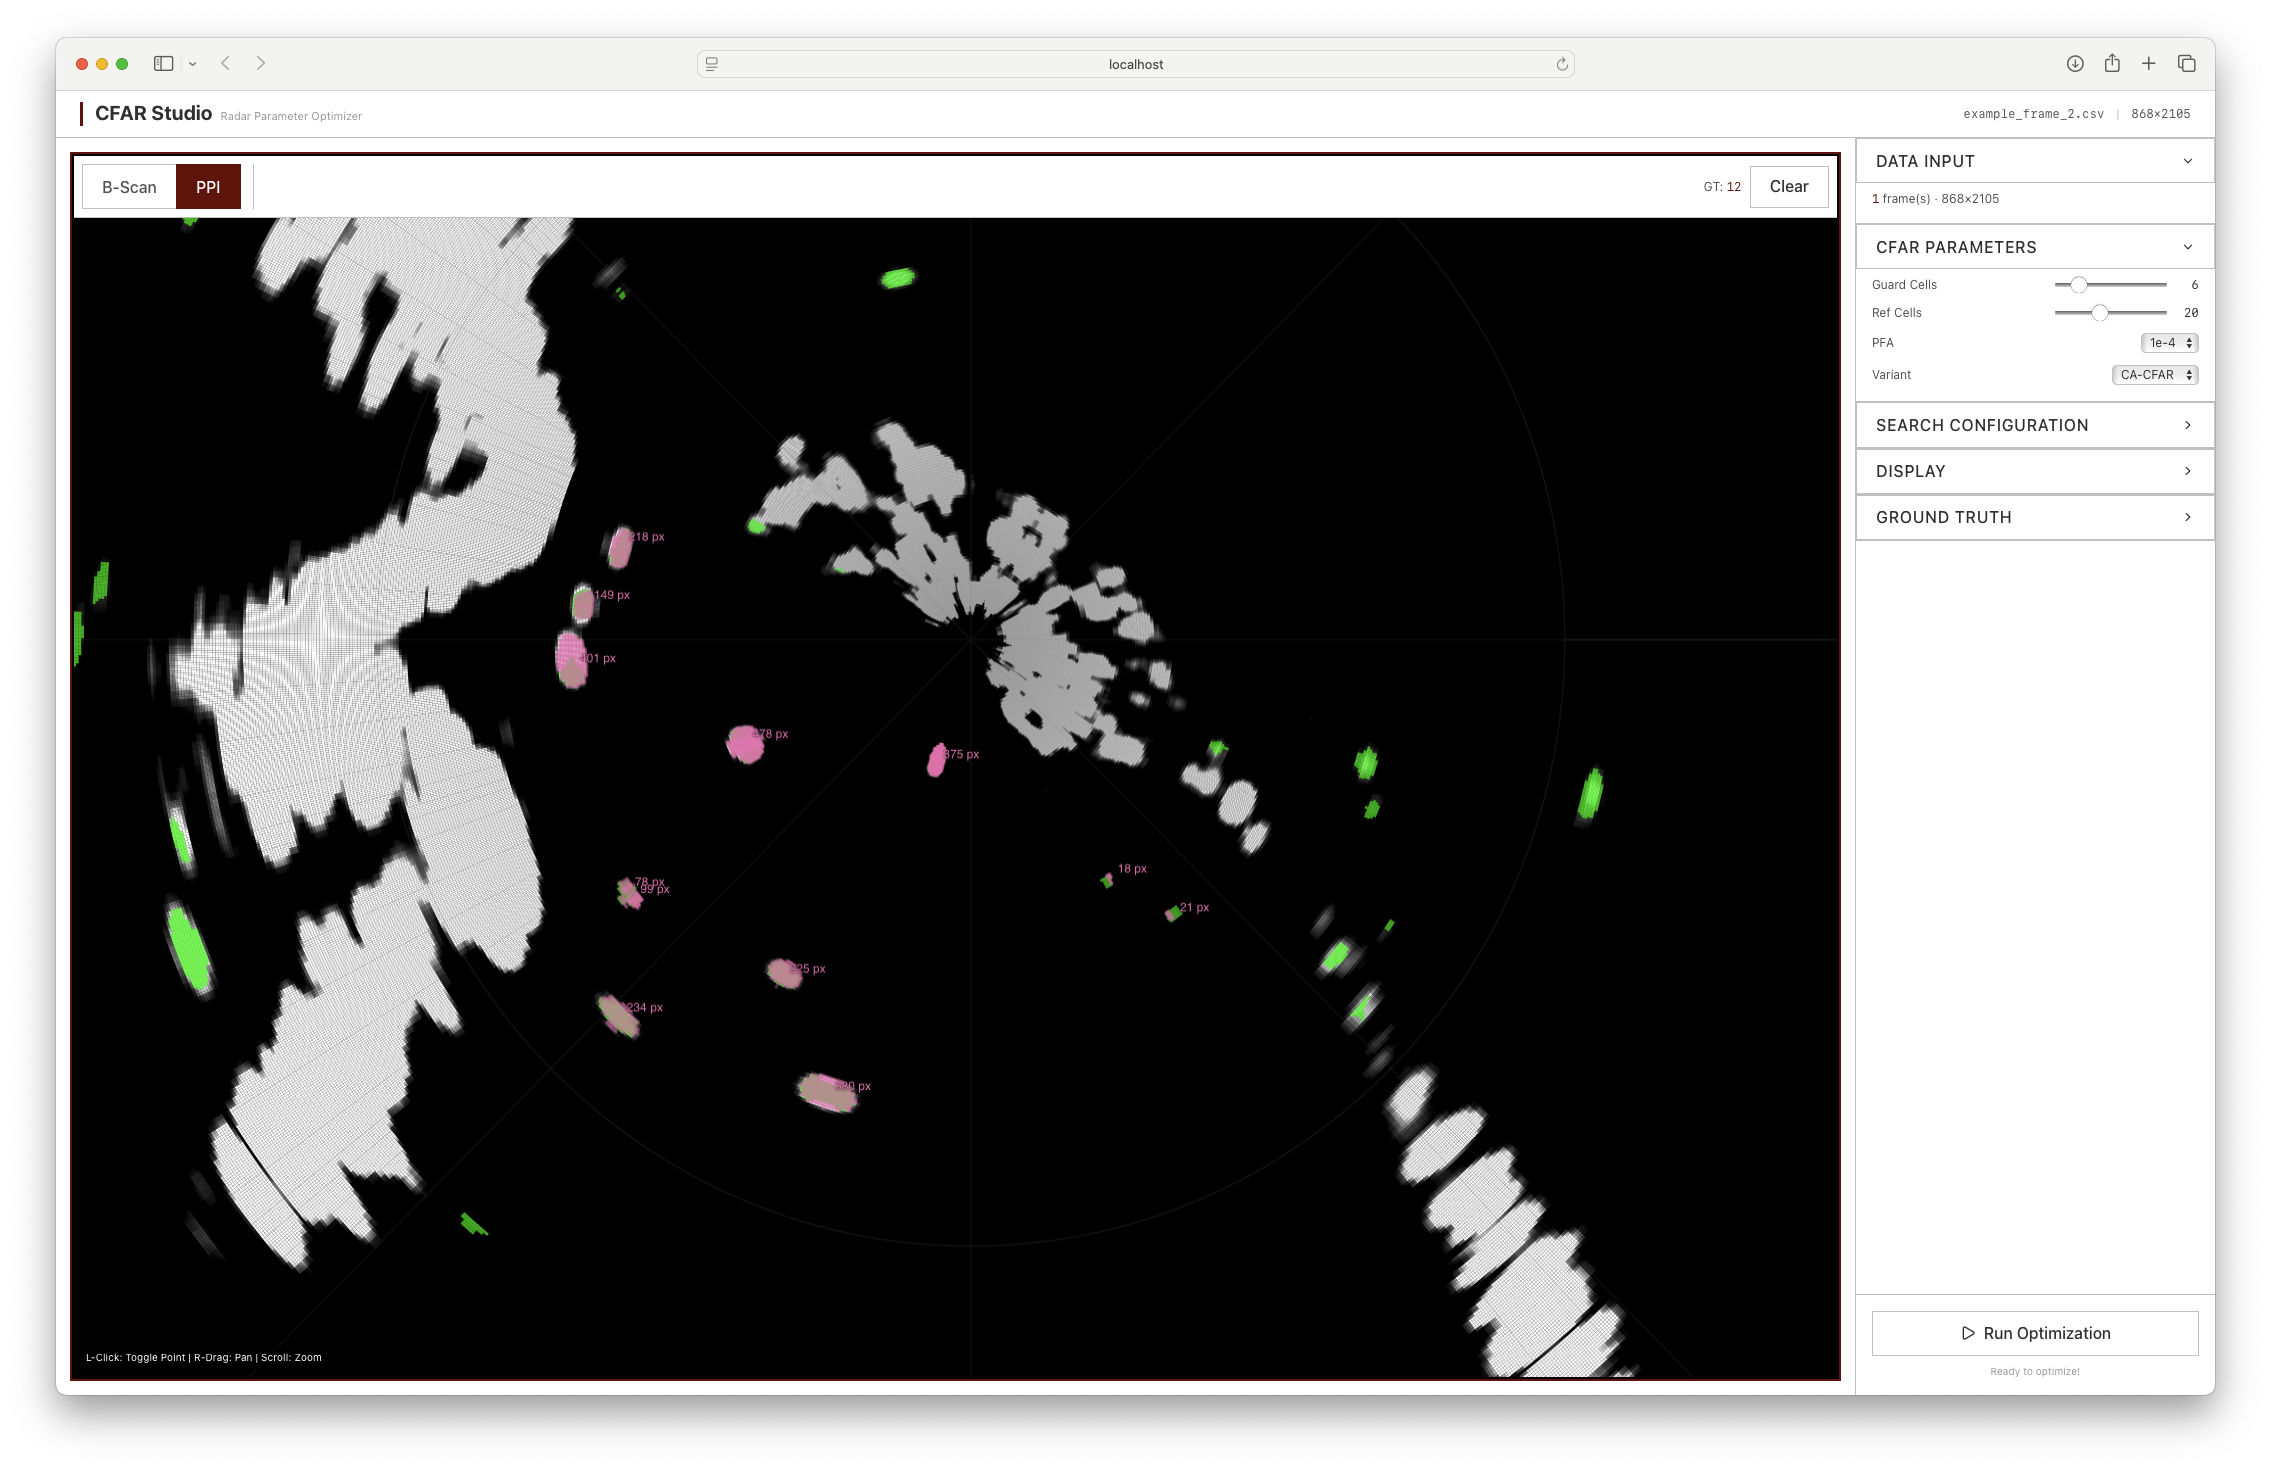
\includegraphics[width=\columnwidth]{figures/ppi_full_view_detections_and_ground_truth.png}
    \caption{PPI display showing raw radar intensity with CFAR detections (highlighted) and annotated ground truth blobs. The overlay enables visual comparison of detection coverage against known targets.}
    \label{fig:ppi_detections}
\end{figure}

The primary display is a PPI view rendered in Cartesian coordinates, with options for multiple colormaps (grayscale, amber, green, inferno, ice). CFAR detections are overlaid as colored highlights, and ground truth annotations are displayed as distinct markers. A B-scan view (Fig.~\ref{fig:bscan}) provides an alternative range--azimuth representation useful for examining clutter structure and detection behavior along individual spokes.

\begin{figure}[t]
    \centering
    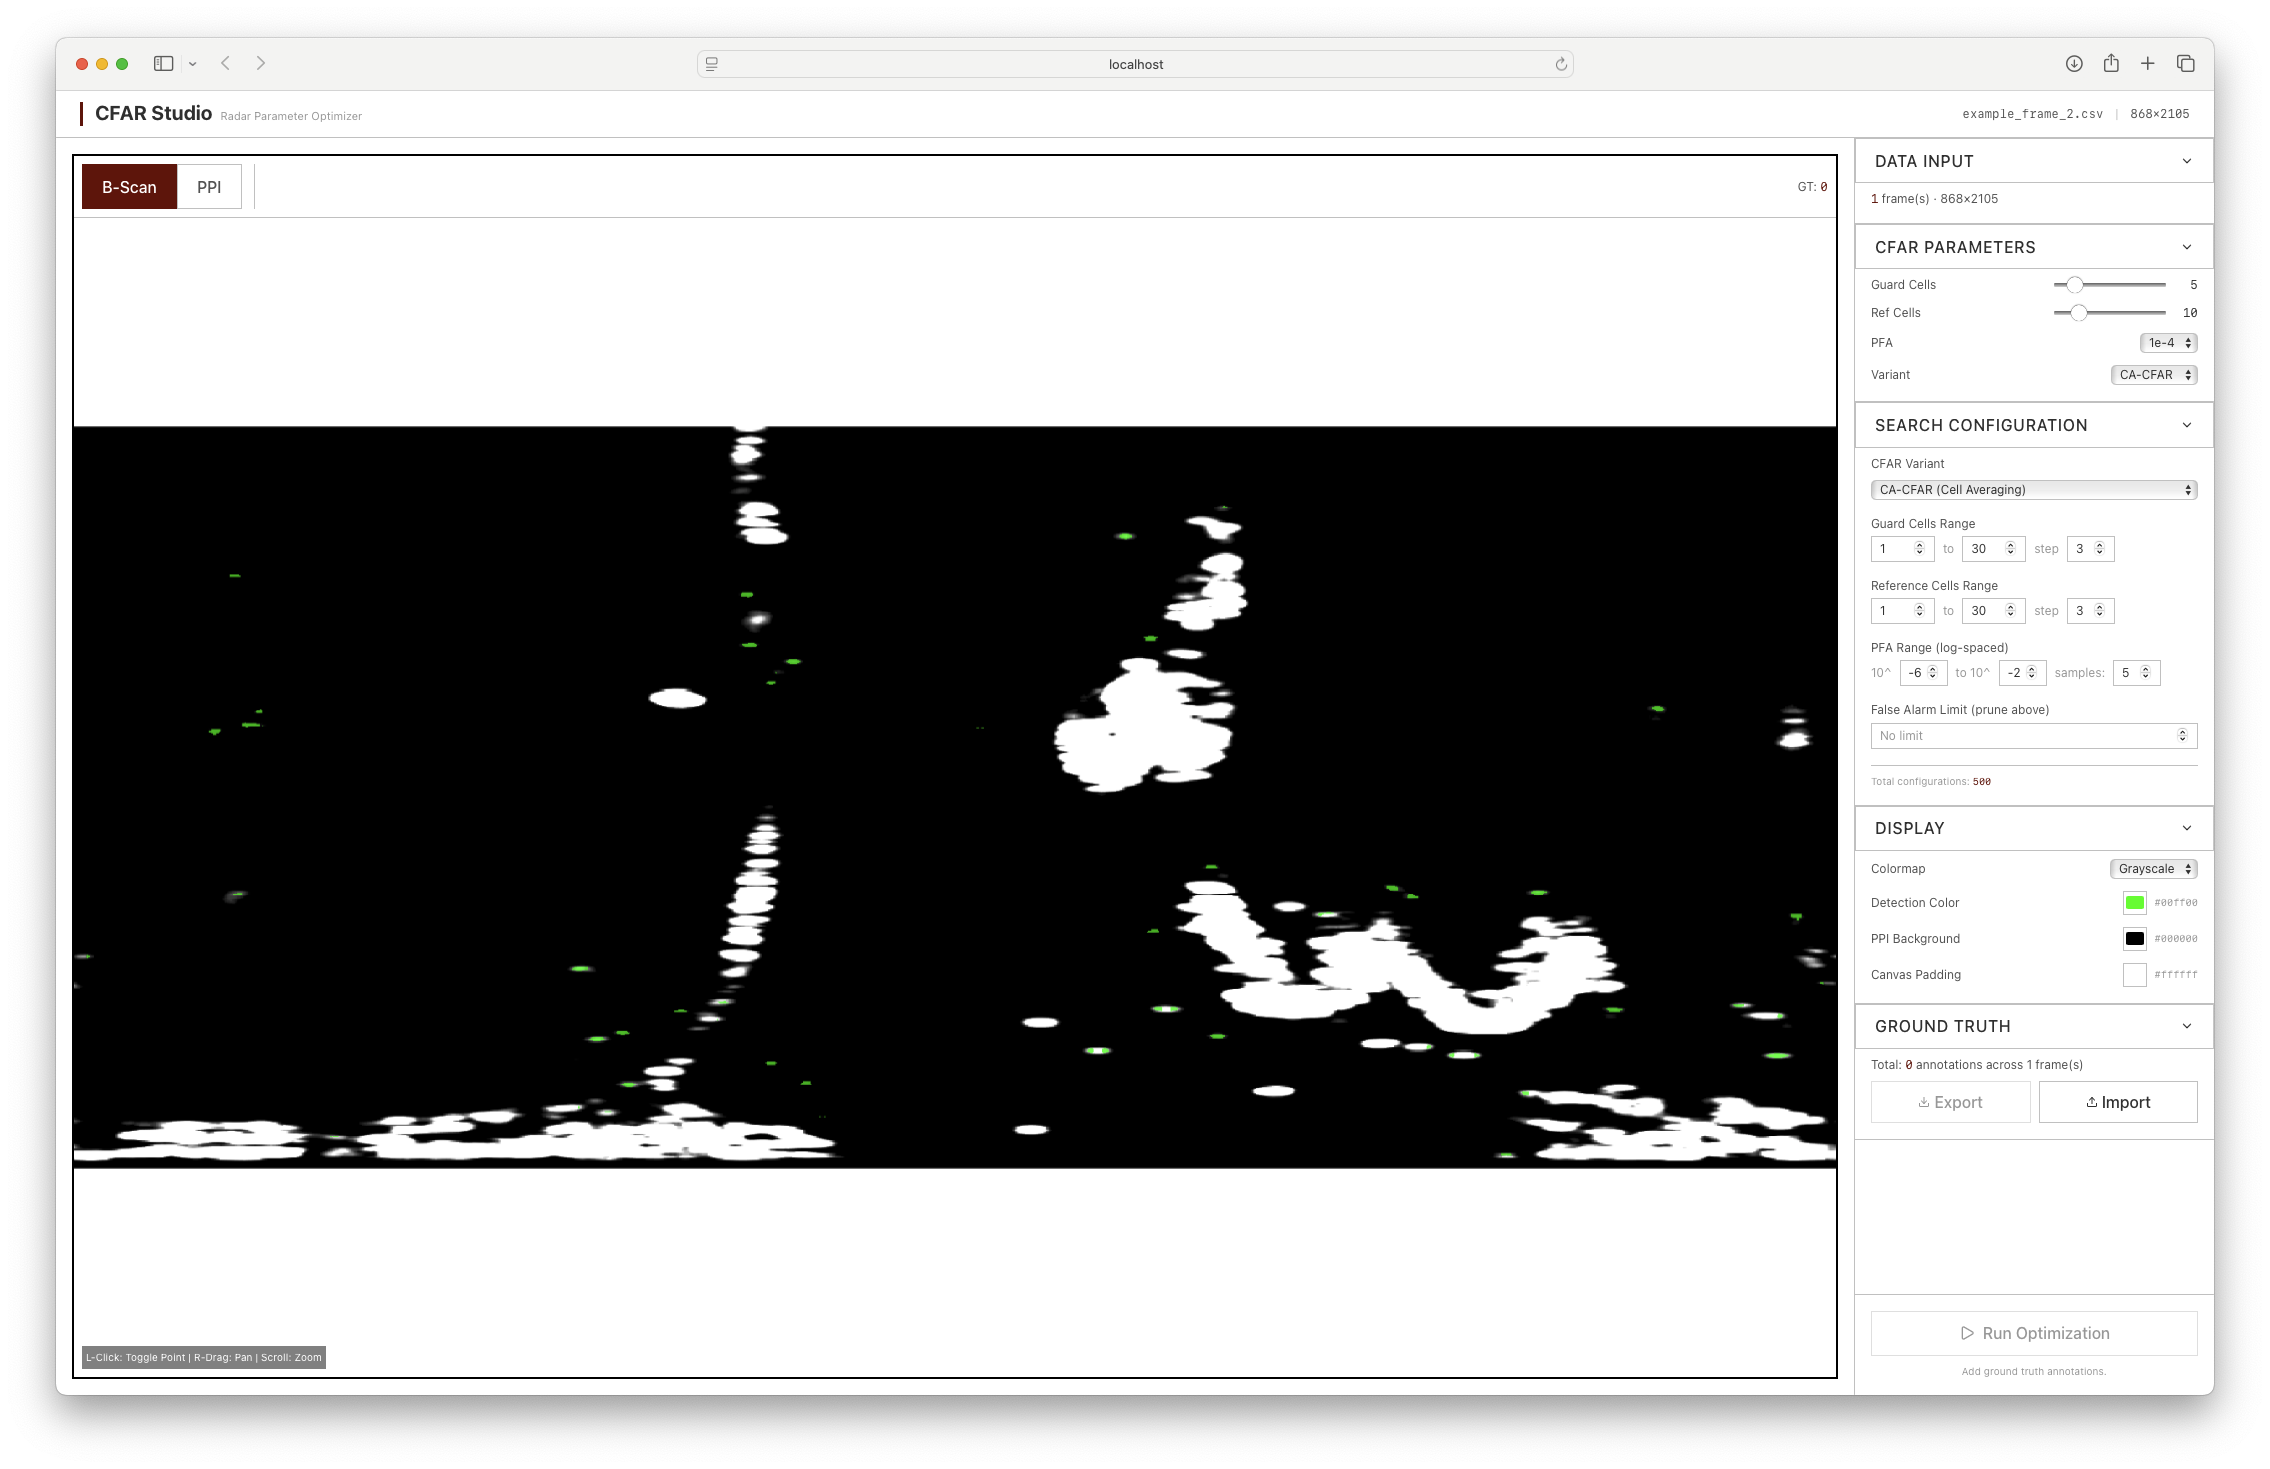
\includegraphics[width=\columnwidth]{figures/bscan_view_grayscale_with_cfar_detections.png}
    \caption{B-scan (range vs.\ azimuth) view with CFAR detections overlaid. This representation reveals clutter structure along individual radar spokes and aids in understanding detection behavior near terrain transitions.}
    \label{fig:bscan}
\end{figure}

The annotation workflow proceeds as follows: (i)~the operator loads radar CSV data and selects CFAR parameters for an initial preview detection; (ii)~on the PPI display, the operator clicks on detected targets representing known stationary objects; (iii)~the system performs an 8-connected flood fill from the click point, tracing the contiguous detection blob and recording all constituent pixel indices as the ground truth reference; (iv)~the blob pixel count is displayed as a size indicator. Ground truth annotations persist across frames, with the assumption that the radar is stationary and reference objects do not move.

When the operator initiates optimization, the parameter ranges (guard cells, reference cells, $P_{\mathrm{FA}}$ values) and CFAR variant are dispatched to a Web Worker. The worker executes Algorithm~\ref{alg:grid_search}, posting progress updates at regular intervals. Upon completion, results are returned to the main thread for visualization in a multi-dimensional results dashboard (Fig.~\ref{fig:full_ui}), including sortable tables, parameter trend plots, and interactive filtering by score, false alarm count, and stability.

\begin{figure*}[t]
    \centering
    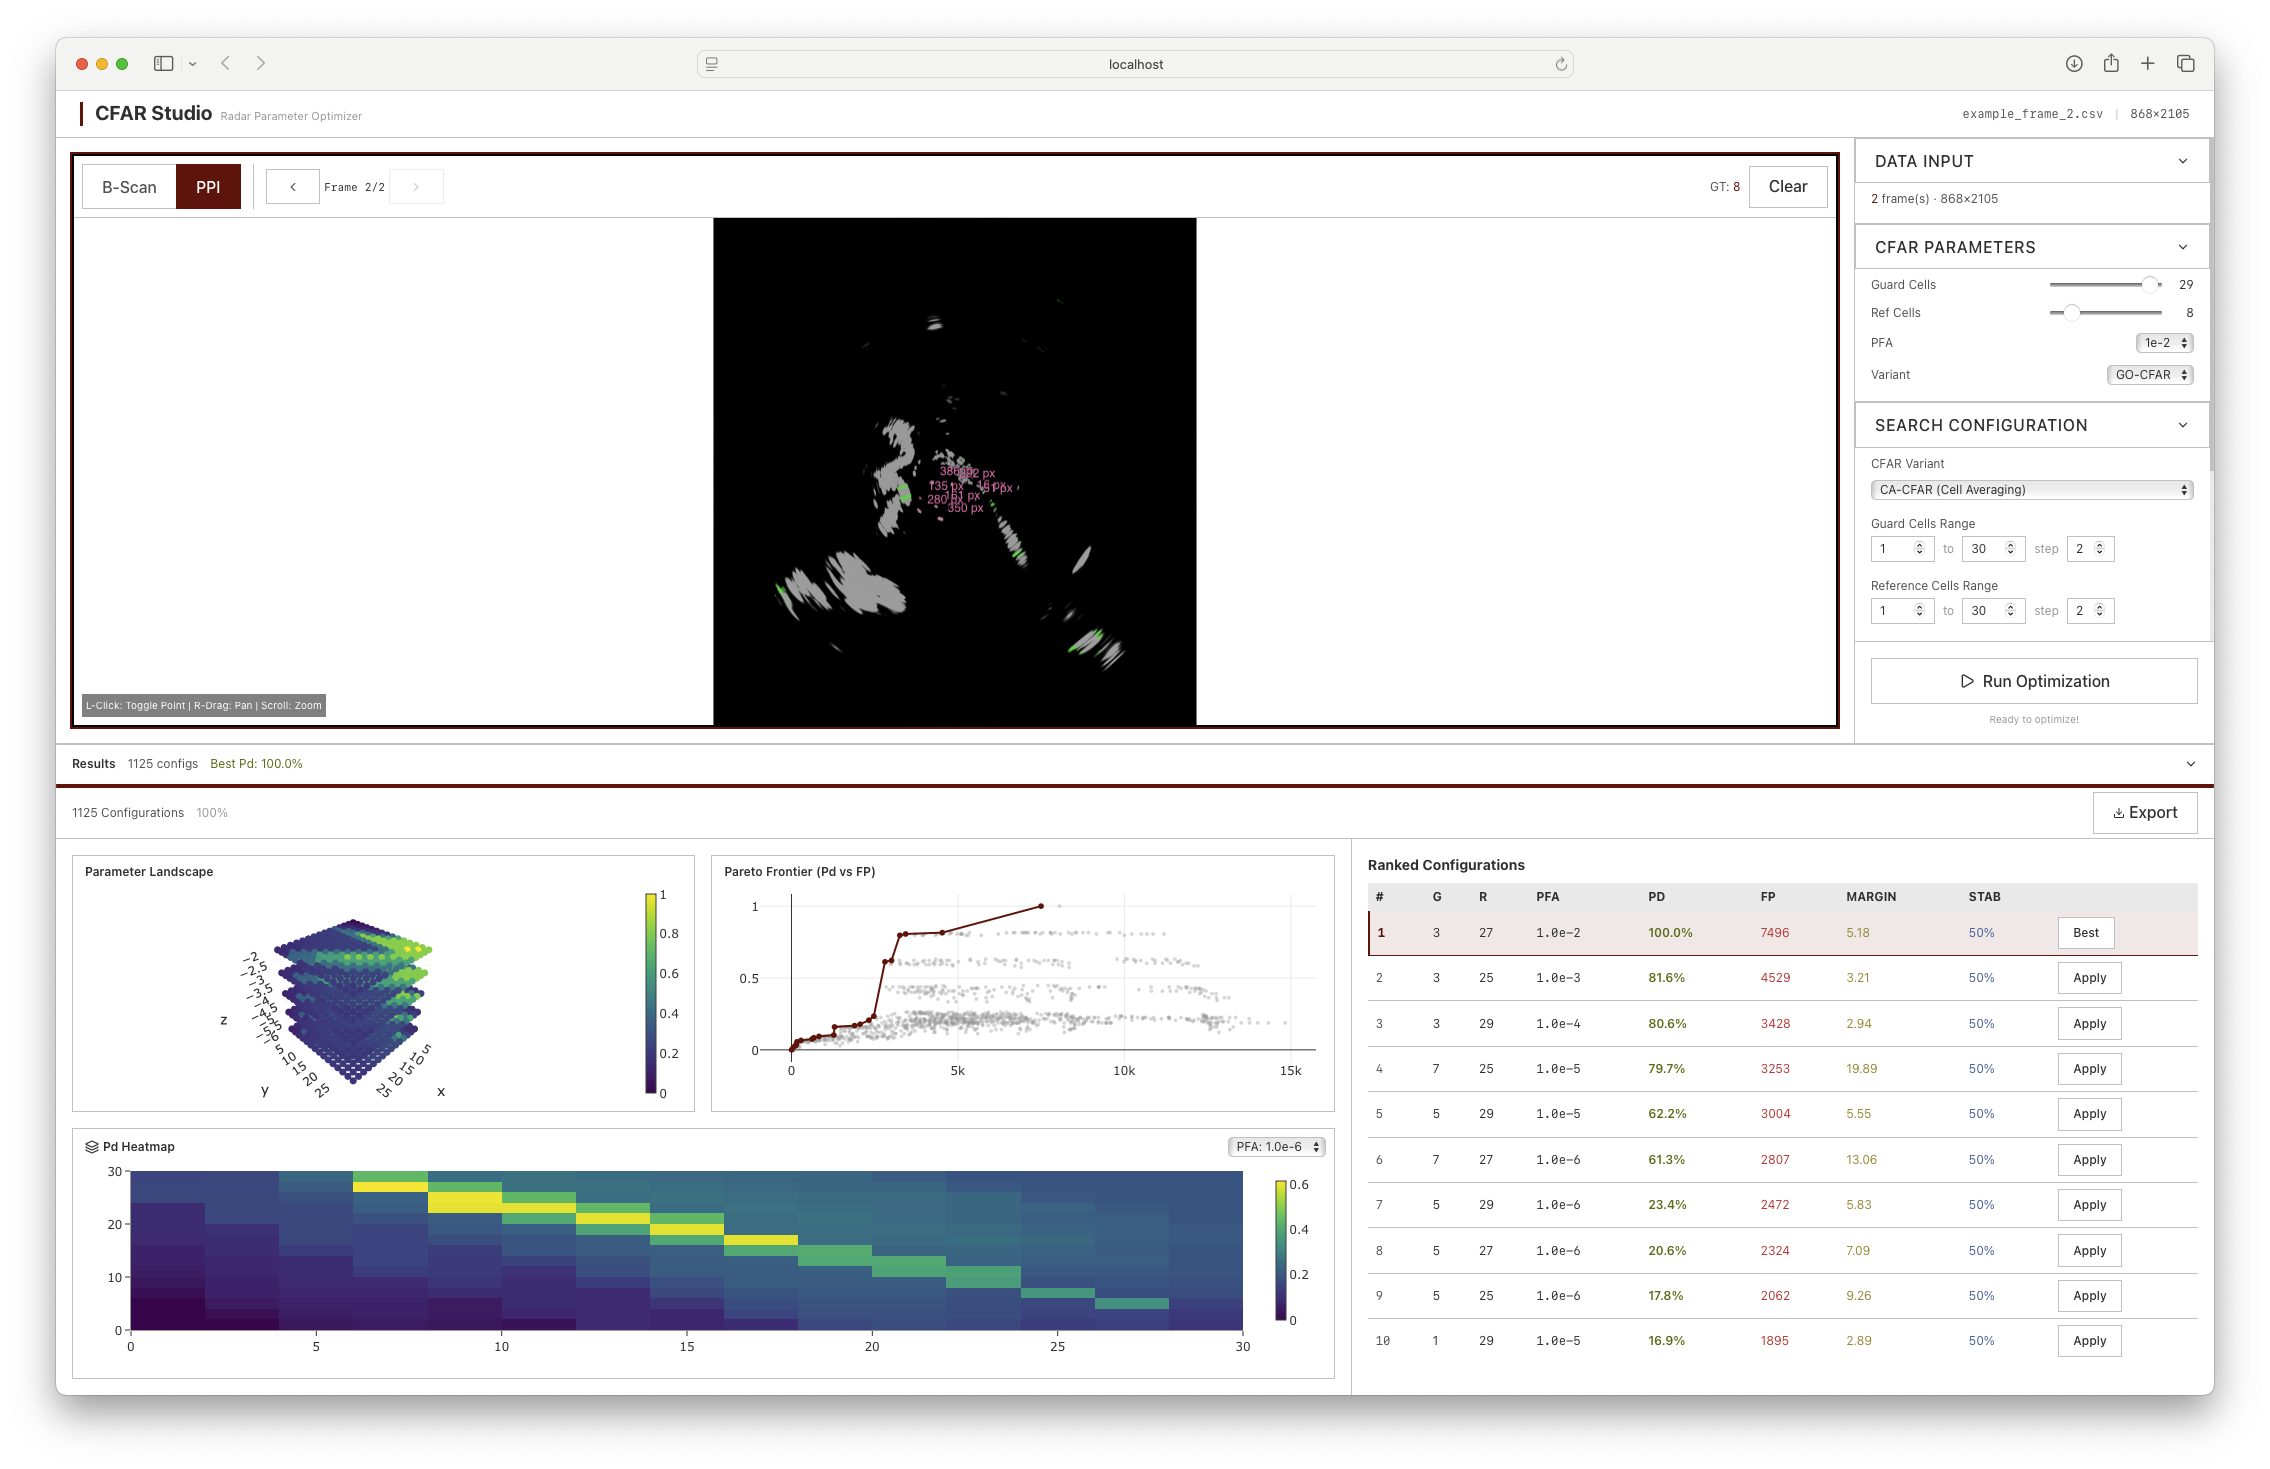
\includegraphics[width=\textwidth]{figures/full_ui_ppi_with_optimization_results.png}
    \caption{Full CFAR Studio interface showing the PPI radar display (left), parameter controls (center), and optimization results dashboard (right) with score rankings and parameter trend visualizations.}
    \label{fig:full_ui}
\end{figure*}

%% ============================================================
%% SECTION 5: EXPERIMENTAL SETUP AND RESULTS
%% ============================================================
\section{Experimental Setup and Results}

Radar data was collected using a Furuno NXT DRS4D X-band (9.41~GHz) solid-state radar connected to a Raspberry Pi~5 single-board computer for raw data digitization and recording. The radar was operated in a shore-based configuration at Lake Murray, Columbia, South Carolina. Lake Murray provides a mixed environment with open water, shoreline structures, and fixed infrastructure -- representative targets for CFAR tuning evaluation.

Raw radar returns were captured as CSV files, with each file representing one complete antenna rotation (360$^\circ$ sweep). Multiple sequential sweeps were recorded to enable multi-frame temporal analysis.

Stationary reference objects were annotated using the blob-tracing tool described in Section~\ref{sec:ground_truth}. Targets included fixed structures and shoreline features that produce consistent radar returns across multiple sweeps. For each target, the operator clicked on the detection under an initial CFAR configuration, and the flood-fill algorithm captured the blob footprint as the ground truth reference.

The grid search swept guard cells $N_g \in [1, 10]$ in steps of 1, reference cells $N_r \in [5, 30]$ in steps of 5, and logarithmically spaced $P_{\mathrm{FA}}$ values in $[10^{-6}, 10^{-2}]$. Each of the three variants (CA, GO, SO) was optimized independently.

A typical grid of approximately 500 parameter configurations completes in under 10 seconds on a modern laptop browser, owing to the integral-image loop hoisting described in Section~\ref{sec:grid_search}.


The optimization results reveal several general trends across the tested CFAR variants. Larger guard cell counts ($N_g \geq 3$) consistently improve scores for extended targets such as dock structures, as they prevent the target's own return from biasing the noise estimate; for point-like targets such as buoys, guard cell sensitivity is lower. Moderate reference window sizes ($N_r \in [10, 20]$) provide the best trade-off between noise estimation accuracy and spatial homogeneity, while very large reference windows ($N_r > 25$) degrade performance near terrain transitions where the training window spans heterogeneous clutter regions.

Lower $P_{\mathrm{FA}}$ values reduce false alarms but risk missing weaker targets. The optimal $P_{\mathrm{FA}}$ depends strongly on the scene -- open-water targets tolerate lower $P_{\mathrm{FA}}$, while targets near clutter edges benefit from moderate $P_{\mathrm{FA}}$ to maintain detection. GO-CFAR tends to produce fewer false alarms near clutter edges at the cost of slightly reduced detection sensitivity, consistent with its conservative noise selection. SO-CFAR provides higher detection rates but generates more false alarms in heterogeneous regions, while CA-CFAR offers a middle ground and often produces the highest overall scores in relatively homogeneous scenes. Across multi-frame sequences, the top-scoring configurations for each variant typically achieve stability values above 0.9, indicating consistent detection of annotated targets across sequential sweeps.

%% ============================================================
%% SECTION 6: DISCUSSION
%% ============================================================
\section{Discussion and Limitations}

The method assumes quasi-stationary reference objects and a fixed radar platform, so that ground truth annotations remain valid across frames. Extension to moving targets or mobile radar platforms would require frame-to-frame registration or track-before-detect association. Running entirely in the browser imposes additional constraints: single-threaded JavaScript execution (mitigated by Web Worker offloading), no GPU acceleration, and a practical file size limit of approximately 50~MB per CSV. For the dataset sizes typical of X-band radar sweeps, these constraints are not limiting.

An exhaustive grid search is computationally feasible for the three-variant, three-parameter space addressed here, with typical grids containing a few hundred configurations evaluable in seconds. More sophisticated approaches such as Bayesian optimization or evolutionary algorithms would become necessary if the parameter space were expanded to include additional CFAR variants with extra parameters (e.g., OS-CFAR order statistic $k$, censoring fractions). The area-weighted coverage score (Eq.~\ref{eq:score_zones}) provides substantially more information than a binary detected/not-detected metric, since a configuration that detects only a small fragment of a large target receives a low score whereas binary scoring would assign full credit. This distinction is important for targets where shape fidelity affects downstream processing such as target classification or extent estimation.

The tool currently supports three CFAR variants (CA, GO, SO); incorporating OS-CFAR or censored variants would require sorting operations that increase per-pixel cost. Data ingestion is limited to the CSV format produced by the Furuno/RPi5 digitization pipeline, and support for additional radar formats would require parser extensions.

Despite these limitations, the framework addresses several operational needs. Rapidly configurable CFAR detection directly improves on-board detection of fixed reference targets during autonomous mapping, approach monitoring and deconfliction, and search-and-rescue operations in cluttered environments where environmental returns generate excessive false alarms. Because the browser-based architecture requires no software installation, no specialized computing hardware, and no network connectivity during operation, an operator can run CFAR Studio on a laptop alongside the radar feed in the field. This zero-infrastructure deployment model is particularly relevant for ad-hoc missions where pre-installed signal processing toolchains are unavailable and radar parameters must be adapted to an unfamiliar scene on short notice.

%% ============================================================
%% SECTION 8: CONCLUSION
%% ============================================================
\section{Conclusion}
We presented CFAR Studio, an open-source, browser-based tool for human-supervised CFAR parameter tuning in heterogeneous radar environments. The system enables an operator to annotate stationary reference objects via blob tracing, then exhaustively searches over three CFAR variants (CA, GO, SO) and their parameter spaces using an integral-image-accelerated grid search. An area-weighted scoring function evaluates each configuration against the annotated ground truth, penalizing partial detections and rewarding full-shape coverage. Multi-frame temporal stability identifies parameter settings that produce consistent detections across sequential radar sweeps.

Demonstrated on real X-band radar data from a Furuno NXT DRS4D at Lake Murray, South Carolina, the tool evaluates hundreds of configurations in seconds within a standard web browser. The results identify scene-specific parameter trends and variant trade-offs that would be difficult to discover through manual trial-and-error tuning. The fully client-side architecture, requiring no installation or server infrastructure, makes the tool suitable for rapid field deployment across a range of radar sensing applications.


\newpage
\begin{thebibliography}{99}
% Note: Page range 414--463 used here; some printings extend to p.~464.
\bibitem{finn1968} H. M. Finn and R. S. Johnson, ``Adaptive detection mode with threshold control as a function of spatially sampled clutter level estimates,'' \emph{RCA Review}, vol.~29, pp.~414--463, Sept.\ 1968. \url{https://www.semanticscholar.org/paper/Adaptive-detection-mode-with-threshold-control-as-a-Finn/1d775905f818bf867029ba6b80ab9974a5566090}

\bibitem{hansen1972} V. G. Hansen and H. R. Ward, ``Detection performance of the cell averaging LOG/CFAR receiver,'' \emph{IEEE Trans.\ Aerosp.\ Electron.\ Syst.}, vol.~AES-8, no.~5, pp.~648--652, Sept.\ 1972. \url{https://doi.org/10.1109/TAES.1972.309580}

\bibitem{trunk1978} G. V. Trunk, ``Range resolution of targets using automatic detectors,'' \emph{IEEE Trans.\ Aerosp.\ Electron.\ Syst.}, vol.~AES-14, no.~5, pp.~750--755, 1978. \url{https://ieeexplore.ieee.org/document/4102054/}

\bibitem{gandhi1988} P. P. Gandhi and S. A. Kassam, ``Analysis of CFAR processors in nonhomogeneous background,'' \emph{IEEE Trans.\ Aerosp.\ Electron.\ Syst.}, vol.~24, no.~4, pp.~427--445, Jul.\ 1988. \url{https://doi.org/10.1109/7.7185}

\bibitem{farina2005review} A. Farina and F. A. Studer, ``A review of CFAR detection techniques in radar systems,'' in \emph{Optimised Radar Processors}, IET, 1987. \url{https://doi.org/10.1049/PBRA001E_ch18}

\bibitem{ward2006} K. D. Ward, R. J. A. Tough, and S. Watts, \emph{Sea Clutter: Scattering, the K Distribution and Radar Performance}. IET, 2006. \url{https://digital-library.theiet.org/doi/book/10.1049/pbra025e}

\bibitem{richards2022} M. A. Richards, \emph{Fundamentals of Radar Signal Processing}, 3rd~ed. McGraw-Hill, 2022. \url{https://www.accessengineeringlibrary.com/content/book/9781260468717}

\bibitem{skolnik2008} M. I. Skolnik, \emph{Radar Handbook}, 3rd~ed. McGraw-Hill, 2008. \url{https://www.accessengineeringlibrary.com/content/book/9780071485470}

\bibitem{crow1984} F. C. Crow, ``Summed-area tables for texture mapping,'' in \emph{Proc.\ ACM SIGGRAPH}, vol.~18, no.~3, pp.~207--212, 1984. \url{https://doi.org/10.1145/800031.808600}

\bibitem{mathworksCFAR} MathWorks, ``Constant False Alarm Rate (CFAR) Detection,'' online documentation, accessed Nov.\ 2025. \url{https://www.mathworks.com/help/phased/ug/constant-false-alarm-rate-cfar-detection.html}

\bibitem{rosenberg2013} L. Rosenberg and S. Bocquet, ``The Pareto distribution for high grazing angle sea-clutter,'' in \emph{Proc.\ IEEE Int.\ Geoscience and Remote Sensing Symp.\ (IGARSS)}, 2013, pp.~4209--4212. \url{https://doi.org/10.1109/IGARSS.2013.6723762}

\bibitem{angelliaume2019} S. Angelliaume, L. Rosenberg, and M. Ritchie, ``Modeling the amplitude distribution of radar sea clutter,'' \emph{Remote Sensing}, vol.~11, no.~3, p.~319, 2019. \url{https://doi.org/10.3390/rs11030319}

\bibitem{humphreys2022} E. Humphreys, M. Antoniou, C. J. Baker, and P. Clark, ``Cognitive CFAR parameter optimization for detection in sea clutter,'' in \emph{Proc.\ Int.\ Conf.\ Radar Syst.\ (RADAR)}, 2022, pp.~148--153. \url{https://doi.org/10.1049/icp.2022.2307}

\bibitem{smith2000} M. E. Smith and P. K. Varshney, ``Intelligent CFAR processor based on data variability,'' \emph{IEEE Trans.\ Aerosp.\ Electron.\ Syst.}, vol.~36, no.~3, pp.~837--847, Jul.\ 2000. \url{https://doi.org/10.1109/7.869503}

\bibitem{nncfar2019} B. P. Rohman and D. Kurniawan, ``Neural network-based adaptive selection CFAR for radar target detection in various environments,'' \emph{Int.\ J.\ Intell.\ Syst.\ Technol.\ Appl.}, vol.~18, no.~4, pp.~377--390, 2019. \url{https://doi.org/10.1504/IJISTA.2019.10021691}

\bibitem{cfarnet2024} T. Diskin, Y. Beer, U. Okun, and A. Wiesel, ``CFARnet: deep learning for target detection with constant false alarm rate,'' \emph{Signal Process.}, vol.~223, p.~109543, 2024. \url{https://doi.org/10.1016/j.sigpro.2024.109543}

\bibitem{seefurther2024} I. Roldan, A. Palffy, J. F. P. Kooij, D. M. Gavrila, F. Fioranelli, and A. Yarovoy, ``See further than CFAR: a data-driven radar detector trained by lidar,'' in \emph{Proc.\ IEEE Radar Conf.\ (RadarConf)}, 2024. \url{https://arxiv.org/abs/2402.12970}

\bibitem{salalstm2023} J. Wang and S. Li, ``SALA-LSTM: a novel high-precision maritime radar target detection method based on deep learning,'' \emph{Scientific Reports}, vol.~13, p.~12125, 2023. \url{https://doi.org/10.1038/s41598-023-39348-3}

\bibitem{farina2008kb} A. De Maio, A. Farina, and G. Foglia, ``Design and experimental validation of knowledge-based constant false alarm rate detectors,'' \emph{IET Radar, Sonar Navig.}, vol.~1, no.~4, pp.~308--316, 2007. \url{https://digital-library.theiet.org/doi/10.1049/iet-rsn:20060113}

\bibitem{wicks1996} M. C. Wicks, W. J. Baldygo, Jr., and R. D. Brown, ``Expert system constant false alarm rate (CFAR) processor,'' U.S.\ Patent 5,499,030, Mar.\ 1996. \url{https://patents.google.com/patent/US5499030}

\bibitem{dhs2009} U.S.\ Dept.\ of Homeland Security, ``Small boat intrusion detection systems with radar,'' System Assessment and Validation for Emergency Responders (SAVER) TechNote, 2009. \url{https://www.dhs.gov/publication/small-boat-intrusion-detection-systems-radar}
\end{thebibliography}

\end{document}
